%Jennifer Pan, August 2011

\documentclass[10pt,letter]{article}
	% basic article document class
	% use percent signs to make comments to yourself -- they will not show up.

\usepackage{amsmath}
\usepackage{amssymb}
\usepackage{tikz}
\usepackage{enumitem}
	% packages that allow mathematical formatting

\usepackage{graphicx}
	% package that allows you to include graphics

\usepackage{setspace}
	% package that allows you to change spacing

\onehalfspacing
	% text become 1.5 spaced

\usepackage{fullpage}
	% package that specifies normal margins

\renewcommand{\vector}[1]{\boldsymbol{#1}}
\newcommand{\problem}[1]{\section*{Problem #1}}
\newcommand{\problempart}[1]{\paragraph{#1}}

\begin{document}
	% line of code telling latex that your document is beginning


\title{Problem Set 5}

\author{Nicholas Wu}

\date{Fall 2020}
	% Note: when you omit this command, the current dateis automatically included

\maketitle
	% tells latex to follow your header (e.g., title, author) commands.
\textbf{Note:} I use bold symbols to denote vectors and nonbolded symbols to denote scalars. I primarily use vector notation to shorthand some of the sums, since many of the sums are dot products.

The first two problems (3, 4) are from the previous problem set.
\problem{3, Problem Set 4}

\problempart{(1)}
\begin{itemize}
  \item The final good producer problem is given by
  \[ \max AL^{1-\alpha} \int_0^{N_t}(x_{j}^\alpha) \ dj - wL - \int_0^{N_t} p_j x_{j} \ dj \]
  The FOC on labor gives
  \[ w = (1-\alpha)AL^{-\alpha) }\int_0^{N_t}(x_{j}^\alpha)  \]
  The FOC on $x_{ji}$ gives
  \[ p_j = \alpha AL^{1-\alpha}x_{j}^{\alpha - 1} \]
  \item The monopolist problem is
  \[ \max \ (\alpha AL^{1-\alpha}x_{j}^{\alpha - 1}) x_{j} - 1 x_{j} \]
  \[ \max \ (\alpha AL^{1-\alpha}x_{j}^{\alpha}) - 1 x_{j} \]
  This has the FOC:
  \[ \alpha^2 AL^{1-\alpha} x_j^{1-\alpha} = 1 \]
  \[ \alpha p_j = 1 \]
  \[ p_j = \alpha^{-1} \]
  So
  \[ x_{jt} = \alpha^{2/(1-\alpha)}A^{1/(1-\alpha)}L \]
  \[ \pi_{jt} = (1-\alpha)\alpha^{(1+\alpha)/(1-\alpha)}A^{1/(1-\alpha)}L \]
  \item The value is given by the Bellman equation:
  \[ r_t V_{jt} - \dot{V}_{jt} = \pi_{jt}  \]
  \item The free entry condition requires $\beta V_j = 1 $.
  \item Then
   \[ r_t/\beta - \dot{V}_{jt} = (1-\alpha)\alpha^{(1+\alpha)/(1-\alpha)}A^{1/(1-\alpha)}L  \]
    \[ r_t = \beta(1-\alpha)\alpha^{(1+\alpha)/(1-\alpha)}A^{1/(1-\alpha)}L  \]
\end{itemize}
\problempart{(2)}
The EE from consumption gives us
\[ \dot{c}/c = \frac{1}{\theta}(r_t-\rho) = g \]

Output is
\[ Y_i = AL_i^{1-\alpha} N x_i^\alpha \]
Net output of the final good is given by
\[ \int_i Y_i = AN \int_i L_i^{1-\alpha} x_i^\alpha \]
\[ = AN \int_i L_i (x_i/L_i)^\alpha \]
Note that $x_i/L_i$ is constant for all firms, since they have the same production function. Hence
\[ = AN \left(x/L\right)^\alpha L \]
\[ = AN x^\alpha L^{1-\alpha} \]
So net output of the final good also grows at the same rate as $N$ and hence as $c$, which is the rate $g$. For $\dot{N} > 0$, we require
\[ \frac{1}{\theta}(r_t-\rho) > 0\]
\[ r_t > \rho \]
\[ \beta(1-\alpha)\alpha^{(1+\alpha)/(1-\alpha)}A^{1/(1-\alpha)}L  > \rho \]
Transversality condition also gives
\[ (1-\theta)g < \rho \]
Plugging in for $r_t$ the growth rate is
\[ g = \frac{1}{\theta}\left(\beta(1-\alpha)\alpha^{(1+\alpha)/(1-\alpha)}A^{1/(1-\alpha)}L-\rho\right) \]
\problempart{(3)}
\begin{itemize}
  \item We need to determine the new interest rate $r'_t$. The altered
  \[ x'_{jt} = \alpha^{2/(1-\alpha)}A^{1/(1-\alpha)}(1-s)L \]
  \[ \pi'_{jt} = (1-\alpha)\alpha^{(1+\alpha)/(1-\alpha)}A^{1/(1-\alpha)}(1-s)L \]
  Applying free-entry to the value function again, we get
  \[ r'_t/\beta = \pi'  \]
  \[ r'_t = \beta (1-\alpha)\alpha^{(1+\alpha)/(1-\alpha)}A^{1/(1-\alpha)}(1-s)L \]
  So the new growth rate is
  \[ g' = \frac{1}{\theta}\left(  \beta (1-\alpha)\alpha^{(1+\alpha)/(1-\alpha)}A^{1/(1-\alpha)}(1-s)L  - \rho \right) \]

  \item Higher $s$ decreases $(1-s)$, which in turn reduces $g'$. This is because higher $s$ reduces the labor force available to the normal non-government firms, and they will do less R\&D and hence the economy growth rate is slower.
  \item The first type of social services might increase overall productivity through $A$, the second type might increase $\beta$ or the effectiveness of research. If $s$ can increase $A$ and $\beta$, then it is possible that higher $s$ can result in sufficient increases in both of these to offset the $(1-s)$ factor. There is room for Pareto improvement in the pricing of $x_j$ goods. Since these are monopolistically priced, the prices are too high and there is inefficiently low usage of the intermediate goods.
\end{itemize}
\pagebreak
\problem{4, Problem Set 4}

\problempart{(1)}
The final good producer FOC in $x_j$ gives
\[ p_j = \alpha x_j^{\alpha - 1}L^{1-\alpha} = \alpha x_j^{\alpha - 1} \]
Then the monopolistic intermediate good producers satisfy
\[ \alpha^2 x_j^{\alpha - 1} = 1 \]
\[ p_j = 1/\alpha \]
So
\[ x_j = \alpha^{2/(1-\alpha)} \]
\[ \pi_j = (p_j - 1) \alpha^{2/(1-\alpha)} = (1-\alpha)\alpha^{(1+\alpha)/(1-\alpha)} \]
Then aggregate output is
\[ Y = A x_j^\alpha = A \alpha^{2\alpha/(1-\alpha)}\]
\[ X = \int_0^A x_j = A\alpha^{2/(1-\alpha)} \]
Assuming investment in research $Z$ is determined,
\[ C = Y - X - Z\]
\problempart{(2)}
The Bellman equation on $V$ is
\[ r_t V - \dot{V} = \pi \]
If there is free entry, $V = \mu$ (the cost of invention). So
\[ r_t \mu = \pi \]
\[ r_t = \mu^{-1}(1-\alpha)\alpha^{(1+\alpha)/(1-\alpha)} \]
The growth rate is then
\[ g = \frac{1}{\theta}(r_t - \rho) = \theta^{-1}(\mu^{-1}(1-\alpha)\alpha^{(1+\alpha)/(1-\alpha)} - \rho) \]
The output growth rate grows at the same rate as consumption, so this is the growth rate of the economy. Then $\mu Z/ A = g$, and assuming $g > 0$ and transversality, this is the equilibrium growth rate.
\problempart{(3)}
Because the monopolist can lose their patent at rate $\xi$, the Bellman equation becomes
\[ (r + \xi)V - \dot{V} = \pi \]
The patent expiry does not affect the monopoly pricing, so $\pi$ is still unchanged, and hence we have
\[ r + \xi = \mu^{-1}(1-\alpha)\alpha^{(1+\alpha)/(1-\alpha)} \]
\[ r = \mu^{-1}(1-\alpha)\alpha^{(1+\alpha)/(1-\alpha)} - \xi \]
The growth rate is then
\[ g = \frac{1}{\theta}(r - \rho) = \theta^{-1}(\mu^{-1}(1-\alpha)\alpha^{(1+\alpha)/(1-\alpha)} - \xi - \rho)\]
Competitive firms charge price $1$, (no profits), so the quantity demanded is $x_j = \alpha^{1/(1-\alpha)}$. Let the measure of monopolistic intermediate good firms be $A_m$, and competitive intermeidate goods be $A_c$. Then we have

\[ Y = A_m x_{jm}^\alpha + A_c x_{jc}^\alpha = A_m \alpha^{2\alpha/(1-\alpha)} + A_c \alpha^{\alpha/(1-\alpha)}\]
\[ X = \int_0^A x_j = A_m \alpha^{2/(1-\alpha)} + A_c \alpha^{1/(1-\alpha)}  \]

\problempart{(4)}
Yes; because all current intermediate goods have no patents, the prices of these goods will be competitively determined and the final good production will be efficient. At the same time, because the government enforces patents going forward, the growth rate in the monopolistic patent case will be maintained because those patents should be respected, and hence the economy will also retain the same rate of innovation. In practice, this may be difficult to believe because doing so may erode trust in the government's enforcement of patents; i.e., inventors may be distrustful of the government's enforcement of patents in the future.
\pagebreak
\problem{1}

\problempart{(1)}
The equilibrium wage and return to capital are determined by the firm's FOCs:
\[w = (3K(0)^{1/2} + L(0)^{1/2})L(0)^{-1/2} = 4 \]
\[R = (3K(0)^{1/2} + L(0)^{1/2})(3K(0)^{-1/2}) = 12 \]
\problempart{(2)}
The equilibrium wage is determined by the firm FOC:
\[ w(t) = (3K(t)^{1/2} + L(t)^{1/2})L(t)^{-1/2} \]
\[ = 3k(t)^{1/2} + 1 \]
The equilibrium labor share is then
\[ \frac{w(t)L(t)}{Y(t)} = \frac{3k(t)^{1/2} + 1}{(3k(t)^{1/2} + 1)^2} = \frac{1}{3k(t)^{1/2} + 1} \]
Yes, the increase in $k(t)$ over time will decrease the equilibrium labor share.
\problempart{(3)}
\begin{enumerate} [label=(\alph*)]
  \item From the Euler condition,
  \[ \frac{c_2(t+1)}{c_1(t)} = \beta R(t+1) \]
  \[ \frac{R(t+1)s(t)}{w(t) - s(t)} = \beta R(t+1) \]
  \[ s(t) = \beta (w(t) - s(t)) \]
  \[ (1+\beta)s(t) = \beta w(t) \]
  \[ s(t) = \frac{\beta}{1+ \beta} w(t) = \frac{\beta}{1+ \beta}\left(3k(t)^{1/2} + 1 \right) \]
  \[ k(t+1)L(t+1) = s(t)L(t) \]
  \[ k(t+1) = (1+n)^{-1} s(t) = \frac{\beta\left(3k(t)^{1/2} + 1 \right)}{(1+ \beta)(1+n)} \]
  and this is our law of motion. For steady state,
  \[ k^* = \frac{\beta\left(3\sqrt{k^*} + 1 \right)}{(1+ \beta)(1+n)} \]
  \[ \frac{(1+ \beta)(1+n)} {\beta} k^* = 3\sqrt{k^*} + 1  \]

  \item Asymptotically, the LHS of our expression in part (a) grows linearly, and the RHS grows at rate $\sqrt{k^*}$. Since at $k^* = 0$, the RHS is greater than the LHS, the LHS asymptotically grows slower than the RHS, and both sides of our expression are monotonically increasing and weakly concave, there can only be one intersection point and hence only one steady state. See figure 1 for relevant diagram.
  \begin{figure}
  \begin{centering}
  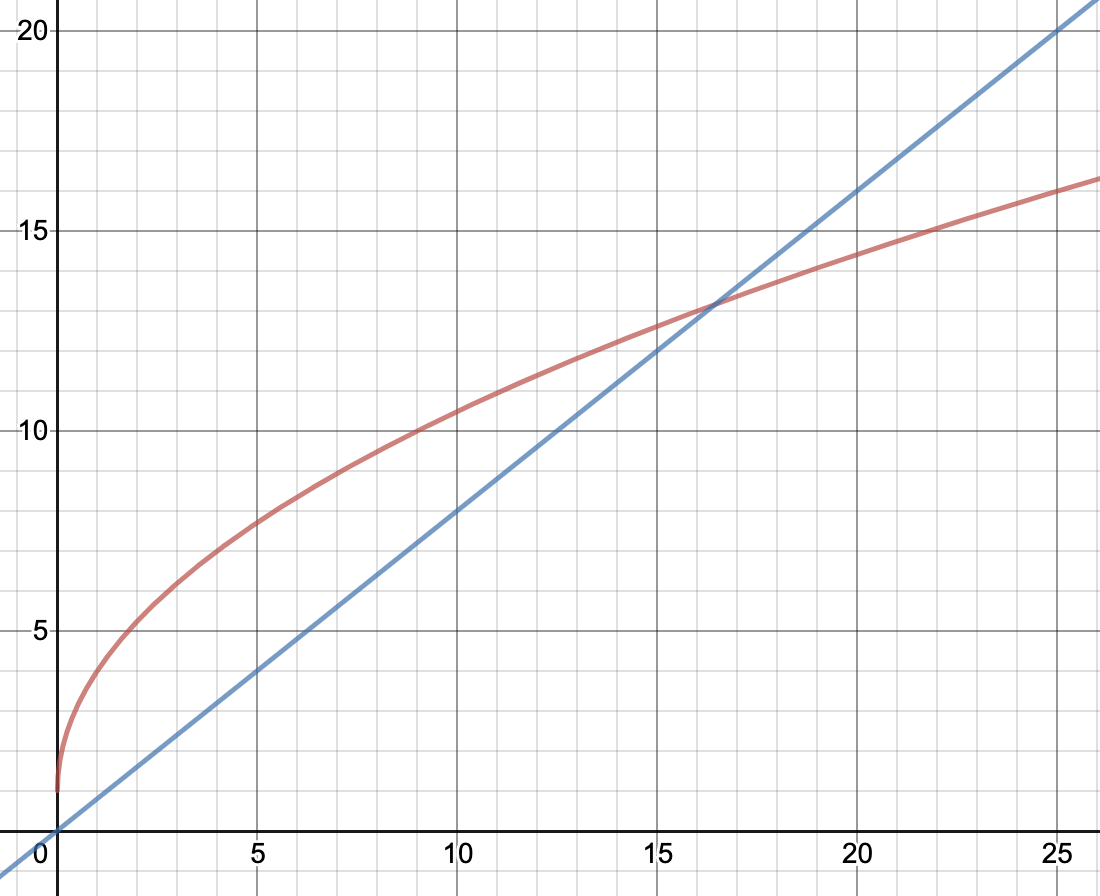
\includegraphics[width=10cm]{ps5fig1}
  \caption{RHS and LHS of steady state determining equation. There can only be one intersection point.}
  \end{centering}
  \end{figure}
  \item Solving for $\beta$, we get
  \[ k^* = \frac{\beta\left(3\sqrt{k^*} + 1 \right)}{(1+ \beta)(1+n)} \]
  \[ k^*(1+n) = \frac{\beta}{1+\beta}\left(3\sqrt{k^*} + 1 \right) \]
  \[ \frac{3\sqrt{k^*} + 1} {k^*(1+n)}=  \frac{1+\beta}{\beta} \]
  \[ \frac{3\sqrt{k^*} + 1} {k^*(1+n)} - 1 = \frac{1}{\beta} \]
  \[ \beta = \frac{1}{\frac{3\sqrt{k^*} + 1} {k^*(1+n)} - 1} = \frac{1}{\frac{3\sqrt{3} + 1} {3(1.0327)} - 1}  \]
  \[ \beta \approx 1.000015 \]
\end{enumerate}
\problempart{(4)}
No dynamic inefficiency means no inefficiency in consumption allocation across generations, from consumers oversaving. To show that this model does not have dynamic inefficiency, we can rewrite the output in terms of $k = K/L$:
\[ f(k) = (3\sqrt{k(t)} + 1)^2 \]
We then note that
\[ f'(k) = \frac{3(3 \sqrt{k(t)}+1)}{\sqrt{k(t)}} = 9 + 3k^{-1/2} \]
\[ r^* = f'(k^*) - 1 = 3(1+ \beta^{-1})\sqrt{k^*}(1+n)  - 1\]
\[= (3(1+ \beta^{-1})\sqrt{k^*}-1) + \left(3(1+ \beta^{-1})\sqrt{k^*} \right)n\]
Let $\alpha = \left(3(1+ \beta^{-1})\sqrt{k^*} \right)$. We note $\alpha \ge 1$, and
\[ r^* = (\alpha - 1) + \alpha n \ge n \]
So there cannot be dynamic inefficiency. The key property is the constant elasticity of substitution between labor and capital.
\problempart{(5)}
No, and the answer does not depend on $\sigma$. Because the funds are reinvested into the capital stock, the funded social security will not decrease savings, and hence cannot lead to Pareto improvement when $r^* < n$. If $\sigma$ is 0, we still have dynamic inefficiency, and increasing $\sigma$ weakly increases net savings, and hence there is no Pareto improvement regardless of the choice of $\sigma$.
\pagebreak
\problem{2}
\problempart{(1)}
The final good producer's problem is
\[ \max 2L^{1/2} \int_0^{N(t)}x(\nu, t)^{1/2}\ d\nu  - w L - \int_0^{N(t)} p^x(\nu, t) x(\nu, t) \  d\nu \]
The wage FOC is
\[w = L^{-1/2} \int_0^{N(t)}x(\nu, t)^{1/2}\ d\nu \]
The intermediate good FOC is
\[ L^{1/2} x(\nu, t)^{-1/2} = p^x(\nu, t) \]
The demand of intermediate inputs is then
\[ x = \frac{L}{(p^x)^{2}} \]
The monopolist pricing on the intermediate input maximizes
\[ \max (p - \psi) x = \frac{L(p-\psi)}{p^2} \]
Taking the FOC, we get
\[ \frac{p^2L - 2pL(p - \psi)}{p^4} = 0 \]
\[ p = 2(p - \psi) \]
\[ p = 2\psi \]
\[ x = \frac{L}{4\psi^2} \]
So the profit is
\[ \pi = (p - \psi)x = \frac{L}{4\psi} \]
Plugging in $\psi = 0.5$, we have
\[ p = 1 \]
\[ x = L \]
\[ \pi = L/2 \]
\[ w = L^{-1/2} \int_0^{N(t)}x(\nu, t)^{1/2}\ d\nu = L^{-1/2} \int_0^{N(t)}L^{1/2}\ d\nu = N \]
and net output is
\[ \hat{Y} = Y - \psi Nx = 2NL - (1/2)NL = (3/2)NL \]

\problempart{(2)}
The firm value function Bellman equation is
\[ r V - \dot{V} = \pi \]
\[ V = \frac{\pi}{r} \]
By free entry, $V = 1$, so $r = \pi = L/2 = 0.05$. So the growth rate is
\[ g = \frac{\dot{c}}{c} = r - \rho = 0.05 - 0.02 = 0.03 \]
\problempart{(3)}
The social planner will price intermediate goods competitively, so $p = \psi$ and $x = L/\psi^2 = 4L$. So net output is $\hat{Y} = 4NL - 2NL = 2NL$. The social planner problem is then
\[ \max \int_0^\infty e^{-\rho t}\log C \ dt \]
subject to
\[ C + Z \le 2NL \]
\[ \dot{N} = Z \]
The present value Hamiltonian is
\[ \log C + \mu(2LN - C) \]
Taking the FOCs:
\[ 1/C = \mu \implies 1 = \mu C \implies \dot{\mu}C = - \dot{C} \mu \implies \frac{\dot{C}}{C} = - \frac{\dot{\mu}}{\mu}\]
\[ 2\mu L = -\dot{\mu} + \rho \mu  \implies -\frac{\dot{\mu}}{\mu} = 2L - \rho\]
so the socially optimal growth rate is $2L - \rho = 0.18$
\problempart{(4)}
In the equilibrium, we have
\[ C = \hat{Y} - Z = 0.15 N - 0.03 N = 0.12 \]
In the socially optimal scenario, we have
\[ C = 2NL - 0.18N = 0.2 - 0.18 = 0.02 \]
The time zero consumption is lower in the socially optimal case, since the research investment for higher growth rate $Z$ is larger than the equilibrium research investment.

\end{document}
	% line of code telling latex that your document is ending. If you leave this out, you'll get an error
